% (c) 2012 Dimitrios Vrettos - d.vrettos@gmail.com
% (c) 2017 Daniele Zambelli - daniele.zambelli@gmail.com
% 
% Tutti i grafici per il capitolo relativo alle relazioni
% 

\newcommand{\insiemes}[4]{% Descrizione della funzione
\begin{tikzpicture}[scale=.7,x=10mm,y=10mm, font=\small, every 
state/.style={draw=CornflowerBlue}, every loop/.style={draw=Maroon}]
\draw (0,0) circle [x radius=3, y radius=2];

\node at (3,1.5) {$S$};
\node[state] (A) at (-2.3,.3) {$A$};
\node[state] (B) at (-.8,1.2) {$B$};
\node[state] (C) at (-1.5,-1) {$C$};
\node[state] (D) at (-.2,-1.1) {$D$};
\node[state] (E) at (.6,.9) {$E$};
\node[state] (F) at (1.8,.5) {$F$};
\node[state] (U) at (1.5,-1) {$U$};

  \begin{scope}[->, Maroon]
 \draw (A)--(U);
  \draw (B)--(C);
 \draw (F)--(U);
   \end{scope}
\end{tikzpicture}
}

\begin{comment}

\newcommand{\nomefunzione}[4]{% Descrizione della funzione
  \def \nomea{#1}
  \def \nomeb{#2}
  \def \nomec{#3}
  \def \nomed{#4}
  \disegno{
  }
}

\end{comment}

\newcommand{\sottoinsiemi}{% Relazione essere sottoinsieme
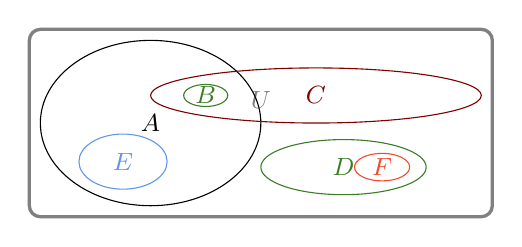
\begin{tikzpicture}[scale=.7, x=10mm, y=10mm, font=\small, every 
state/.style={draw=CornflowerBlue}, every loop/.style={draw=Maroon}]
\draw (-2.2, -1.7) [very thick, gray, rounded corners] rectangle (6.2, 1.7) 
      node [midway, above=1.2] {$U$};
\draw (0,0) circle [orange!50!black, x radius=2, y radius=1.5] node {$A$};
\draw[CornflowerBlue] (-.5,-.7) circle [x radius=.8, y radius=.5]node {$E$};
\draw[OliveGreen] (1,.5) circle [x radius=.4, y radius=.2]node {$B$};
\draw[Maroon] (3,.5) circle [x radius=3, y radius=.5]node {$C$};
\draw[OliveGreen] (3.5,-.8) circle [x radius=1.5, y radius=.5]node {$D$};
\draw[RedOrange] (4.2,-.8) circle [x radius=.5, y radius=.25]node {$F$};
% 
% \node () at (2.1,2) {$U$};
\end{tikzpicture}
}

\newcommand{\relsottoinsieme}{% Relazione essere sottoinsieme
\begin{tikzpicture}[scale=.7,x=10mm,y=10mm, font=\small, every 
state/.style={draw=CornflowerBlue}, every loop/.style={draw=Maroon}]
\draw (0,0) circle [x radius=3, y radius=2];

\node at (3,1.5) {$S$};
\node[state] (A) at (-2.3,.3) {$A$};
\node[state] (B) at (-.8,1.2) {$B$};
\node[state] (C) at (-1.5,-1) {$C$};
\node[state] (D) at (-.2,-1.1) {$D$};
\node[state] (E) at (.6,.9) {$E$};
\node[state] (F) at (1.8,.5) {$F$};
\node[state] (U) at (1.5,-1) {$U$};

  \begin{scope}[->, Maroon]
 \draw (A)--(U);
  \draw (B)--(C);
 \draw (F)--(U);
   \end{scope}
\end{tikzpicture}
}
% 
% \newcommand{\grafoscatoladx}[4]{% 
%   % Funzione unaria rappresentata come scatola nera a destra
%   % esempio di chiamata:
%   % \grafoscatoladx{add}{\7\)}{\(5\)}{\(12\)}
%   \def \nomef{#1}
%   \def \opa{#2}
%   \def \opb{#3}
%   \def \risultato{#4}
%   \disegno[10]{
%      \node [draw, fill=blue!20, minimum size=3em, rounded corners] 
%             at (0, 2) (block 2) {\nomef};
%      \draw [->] (1, 1.5) node [right] {\opa} -- (block 2);
%      \draw [->] (1, +2.5) node [right] {\opb} -- (block 2);
%      \draw[->] (block 2.west) -- (-1, 2) node [left] {\risultato};
%   }
% }

\newcommand{\grafifunzbinarie}{% Grafi di alcune funzioni su coppie di numeri
  \disegno[10]{
  \grafofunzsx{add}{\(\graffa{+7,~+5}\)}{\(+12\)}
  \begin{scope}[xshift=50mm]
  \grafofunzsx{sub}{\(\tonda{+7,~+5}\)}{\(+2\)}
  \end{scope}
  \begin{scope}[xshift=100mm]
  \grafofunzsx{sub}{\(\tonda{+5,~+7}\)}{\(-2\)}
  \end{scope}
  }
}

\newcommand{\grafidivisione}{% Grafi di divisione
  \disegno[10]{
  \grafofunzsx{div}{\(\tonda{+7,~+3}\)}{\(+2\)}
  \begin{scope}[xshift=50mm]
  \grafofunzsx{div}{\(\tonda{+7,~+3}\)}{\(+\dfrac{7}{3}\)}
  \end{scope}
  }
}

\newcommand{\grafidivmod}{% due esempi della funzione divmod
  \disegno[10]{
  \grafofunzsx{divmod}{\(\tonda{+7,~+3}\)}{\(\tonda{+2,~1}\)}
  \begin{scope}[xshift=50mm]
  \grafofunzsx{divmod}{\(\tonda{+7,~0}\)}{Errore}
  \end{scope}
  }
}

\newcommand{\arcofunzione}[4]{% Traccia una freccia tra due nodi
  \def \posa{#1}
  \def \labela{#2}
  \def \posb{#3}
  \def \labelb{#4}
  \node at \posa (a) {\(\labela\)};
  \node at \posb (b) {\(\labelb\)};
  \draw [-angle 60] (a.east) .. controls +(30:1cm) and +(150:.5cm) .. 
                    (b.west);

}

\newcommand{\funzdivmod}{
% Grafi di Elero per rappresentare la funzione div
  \disegno[10]{
    \node [very thick, green!50!black]at (0, 2.1) {div};
    \draw [very thick, blue!50!black] 
          (-2, 0) circle[ x radius=1.5, y radius=2.1, rotate=+30]
          node at (-3, -1.6) {\(A\)};
    \draw [very thick, CornflowerBlue!50!black]
          (-2.3, 0.5) circle[ x radius=1.2, y radius=1.4, rotate=+20]
          node at (-2.6, -1.0) {\(ID\)};
    \draw [very thick, red!50!black] 
          (+2, 0) circle[ x radius=1.5, y radius=2.1, rotate=-30]
          node at (+3, -1.6) {\(B\)};
%     \node at (+3, -1.6) {\(B\)};
    \draw [very thick, orange!70!black] 
          (+2.3, 0.5) circle[ x radius=1.2, y radius=1.4, rotate=-10]
          node at (+2.5, -1.1) {\(IM\)};
    \arcofunzione{(-2.4, 1.4)}{\tonda{7,~3}}{(+2.2, 1.4)}{\dfrac{7}{3}}
    \arcofunzione{(-2.7, 0.8)}{\tonda{18,~6}}{(+1.8, 1.0)}{3}
    \arcofunzione{(-2.8, 0.2)}{\tonda{5,~4}}{(+2.6, 0.4)}{\dfrac{5}{4}}
    \arcofunzione{(-2.6, -0.4)}{\tonda{2,~8}}{(+2.1, -0.1)}{\dfrac{1}{4}}
    \node at (-1.2, -1.1) {\(\tonda{6,~0}\)};
    \node at (-1.7, -1.6) {\(\tonda{0,~0}\)};
    \node at (1.1, -1.1) {\(\dfrac{6}{5}\)};
    \node at (1.8, -1.6) {\(4\)};
  }
}

\newcommand{\esefunz}{
% Grafi di Elero per rappresentare la funzione 1/x^2
  \disegno[10]{
    \node [very thick, green!50!black]at (0, 2.1) {div};
    \draw [very thick, blue!50!black] 
          (-2, 0) circle[ x radius=1.5, y radius=2.1, rotate=+30]
          node at (-3, -1.6) {\(D\)};
    \draw [very thick, CornflowerBlue!50!black]
          (-2.2, 0.2) circle[ x radius=1.2, y radius=1.6, rotate=+20]
          node at (-2.1, -1.55) {\(ID\)};
    \draw [very thick, red!50!black] 
          (+2, 0) circle[ x radius=1.5, y radius=2.1, rotate=-30]
          node at (+3, -1.6) {\(C\)};
%     \node at (+3, -1.6) {\(B\)};
    \draw [very thick, orange!70!black] 
          (+2.3, 0.0) circle[ x radius=1.0, y radius=1.0, rotate=-10]
          node at (+2.5, -1.2) {\(IM\)};
    \arcofunzione{(-2.4, +1.4)}{-3}{(+2.2, +0.5)}{\dfrac{1}{9}}
    \arcofunzione{(-2.4, -0.6)}{+3}{(+2.2, +0.5)}{\quad}
    \arcofunzione{(-2.6, +1.0)}{-2}{(+1.9, -0.45)}{\dfrac{1}{4}}
    \arcofunzione{(-2.6, -0.2)}{+2}{(+1.9, -0.45)}{\quad}
    \arcofunzione{(-2.7, +0.6)}{-1}{(+2.8, -0.05)}{1}
    \arcofunzione{(-2.7, +0.2)}{+1}{(+2.8, -0.05)}{~}
    \node at (-1.3, -1.6) {\(0\)};
    \node at (2.2, +1.5) {\(-3\)};
    \node at (1.8, +1.2) {\(-2\)};
    \node at (1.2, -1.2) {\(\dfrac{5}{6}\)};
    \node at (1.7, -1.5) {\(0\)};
    \node at (-2.0, -1.0) {\dots};
    \node at (+3.0, +1.1) {\dots};
    \node at (+2.5, -0.7) {\dots};
  }
}

\newcommand{\deffunzione}[4]{% 
  % Definizione di funzione
  \def \nomea{#1}
  \def \nomeb{#2}
  \def \nomec{#3}
  \def \nomed{#4}
  \disegno[4]{
    \shadedraw [shading=ball]
      (0,0) circle [x radius=2, y radius=3, ball color=red!20, rotate=+20];
    \draw [red!0, dashed]
          [postaction={decoration={text along path, text={\nomeb},
           text align={align=center}}, decorate}]
          (-2.5,1) .. controls (-2,4) and (1,4) .. (2,1);
    \shadedraw[
      top color=yellow!70,
      bottom color=red!70,
      shading angle={45},
      opacity=.5,
      x radius=4, y radius=5] (0, 0) circle; 
    \draw [red!0, dashed]
          [postaction={decoration={text along path, text={\nomea},
           text align={align=center}}, decorate}]
      (-3.5,3) .. controls (-2,6) and (2,6) .. (3.5,3);
    \shadedraw [shading=ball] (12,0) circle [x radius=1.6, y radius=2.4,
                                           ball color=red!20, rotate=-20];
    \draw [red!0, dashed]
          [postaction={decoration={text along path, text={\nomed},
           text align={align=center}}, decorate}]
          (10.2,.5) .. controls (11,3.5) and (14,3.5) .. (14,.5);
    \shadedraw[
      top color=yellow!70,
      bottom color=blue!70,
      shading angle={45},
      opacity=.5,
      x radius=4, y radius=5] (12, 0) circle;
    \draw [red!0, dashed]
          [postaction={decoration={text along path, text={\nomec},
           text align={align=center}}, decorate}]
      (8.5,3) .. controls (10,6) and (14,6) .. (15.5,3);
    \draw [|->, very thick] (0, 0) to [out=20, in=160,
       edge node={node [sloped,above] {\(f\)}}] (12, 0);
    \draw (-1, 2.824) to [out=20, in=160] (12.8, 2.26);
    \draw (+1.1,-2.8) to [out=20, in=160] (11.2,-2.27);
  }
}

\newcommand{\funzcostante}{
% Grafi di Elero per rappresentare la funzione 1/x^2
  \disegno[10]{
    \node [very thick, green!50!black]at (0, 2.1) {\(f\)};
    \draw [very thick, blue!50!black] 
          (-2, 0) circle[ x radius=1.5, y radius=2.1, rotate=+30]
          node at (-3, -1.6) {\(D\)};
    \draw [very thick, CornflowerBlue!50!black]
          (-2.2, 0.0) circle[ x radius=1.2, y radius=1.8, rotate=+20]
          node at (-1.0, -1.6) {\(ID\)};
    \draw [very thick, red!50!black] 
          (+2, 0) circle[ x radius=1.5, y radius=2.1, rotate=-30]
          node at (+3, -1.6) {\(C\)};
%     \node at (+3, -1.6) {\(B\)};
    \draw [very thick, orange!70!black] 
          (+2.4, 0.0) circle[ x radius=0.8, y radius=0.6, rotate=+20]
          node at (+2.8, -0.8) {\(IM\)};
    \arcofunzione{(-2.4, +1.4)}{a}{(+2.8, -0.05)}{\quad}
    \arcofunzione{(-2.0, -1.5)}{g}{(+2.8, -0.05)}{\quad}
    \arcofunzione{(-2.6, +0.9)}{b}{(+2.8, -0.05)}{\quad}
    \arcofunzione{(-2.4, -1.1)}{f}{(+2.8, -0.05)}{\quad}
    \arcofunzione{(-2.7, +0.4)}{c}{(+2.8, -0.05)}{-2}
    \arcofunzione{(-2.7, -0.6)}{e}{(+2.8, -0.05)}{\quad}
    \arcofunzione{(-2.5, -0.1)}{d}{(+2.8, -0.05)}{\quad}
    \node at (2.2, +1.6) {\(-3\)};
    \node at (1.8, +1.2) {\(-1\)};
    \node at (2.6, +1.0) {\(0\)};
    \node at (1.7, -1.5) {\(+1\)};
    \node at (1.2, -1.0) {\(+2\)};
    \node at (2.0, -1.1) {\(+3\)};
  }
}

